\documentclass[final]{beamer}
\usepackage[size=a0,orientation=portrait,scale=1.0]{beamerposter}
\usepackage{graphicx}
\usepackage{lmodern} % for better fonts
\usepackage{tikz}
\usepackage{multicol}
\usepackage{wrapfig}

% Color scheme
\definecolor{maincolor}{RGB}{0, 70, 140}  % Deep blue
\definecolor{lightgray}{RGB}{240,240,240}

% Poster settings
\title{Hacking on the Software Stack at VSC}
\author{Adam McCartney, Luis Casillas-Trujillo, Filip Kocina, Moritz Siegel
\quad | \quad VSC Research Center}
\date{\today}

\setbeamercolor{block title}{fg=white,bg=maincolor}
\setbeamercolor{block body}{fg=black,bg=white}
\setbeamercolor{background canvas}{bg=lightgray}


%%%%%%%%%%%%%%%%%%%%%%%%%%
% code snippet setup
%%%%%%%%%%%%%%%%%%%%%%%%%%
\usepackage{listings}
\usepackage{xcolor}

\lstset{
  basicstyle=\ttfamily\small,
  backgroundcolor=\color{white},
  frame=single,
  rulecolor=\color{gray},
  keywordstyle=\color{blue},
  commentstyle=\color{gray},
  stringstyle=\color{orange},
  breaklines=true,
  showstringspaces=false,
  tabsize=2,
  captionpos=b
}


\begin{document}
\begin{frame}[t]

% Title
\begin{center}
  \vspace{1cm}
  \usebeamercolor[fg]{title}
  \Huge \textbf{\inserttitle}
  
  \vspace{0.5cm}
  \Large \insertauthor
  
  \vspace{1cm}
\end{center}

%%%%%%%%%%%%%%%%%%%%%%%%%%%%%%%%%
% Begin content
%%%%%%%%%%%%%%%%%%%%%%%%%%%%%%%%%
\begin{columns}[t]
  \begin{column}{0.48\textwidth}
    \begin{block}{Introduction}
     \begin{itemize}
      \item The evolution of the software stack followed key stages:
      \begin{itemize}
        \item \textbf{VSC 1–2}: Software installed manually by expert users.
        \item \textbf{VSC 3–4}: Managed by custom scripts; more structure introduced.
        \item \textbf{VSC 4–5}: Adoption of Spack allowed faster installation and automatic dependency handling.
      \end{itemize}
      \item Challenges
      \begin{itemize}
        \item Complex software presentation.
        \item Unresolved issues around deduplication.
        \item Organizational strain during OS upgrades with little test coverage.
        \item \textbf{MUSICA} introduces the need to distribute software across sites.
      \end{itemize}
     \end{itemize}
    \end{block}
    \vfill

    \begin{block}{Methods}
        \begin{itemize}
          \item In 2024, the \textbf{Software and Modules (SAM)} starts to explore solutions.
          \item October - December 2024, evaluation of: Guix, Nix, Spack, EasyBuild, EESSI, Lmod, and ReFrame.
          \item Early 2025, two contrasting strategies were implemented on the new \textbf{MUSICA} cluster:
          \begin{itemize}
            \item \textbf{EESSI on the side}: Host-based installs using EasyBuild and the \texttt{sse2} toolkit, with limited EESSI integration.
            \item \textbf{EESSI as a base}: All software build will be integrated into EESSI's compatibility layer.
                \begin{itemize}
                  \item \texttt{EESSI\_USER\_INSTALL}
                  \item \texttt{EESSI\_SITE\_INSTALL}
                  \item \texttt{EESSI\_PROJECT\_INSTALL} to \texttt{/cvmfs/software.asc.ac.at}
                \end{itemize}
          \end{itemize}
          \item Test stack: AOCC, Intel compilers, NVHPC, VASP 6.5.0 (CPU \& GPU), Mathematica, Containers.

        \end{itemize}
    \end{block}
    \vfill

    \begin{block}{Distribution across sites possible with CVMFS}
      \begin{center}
        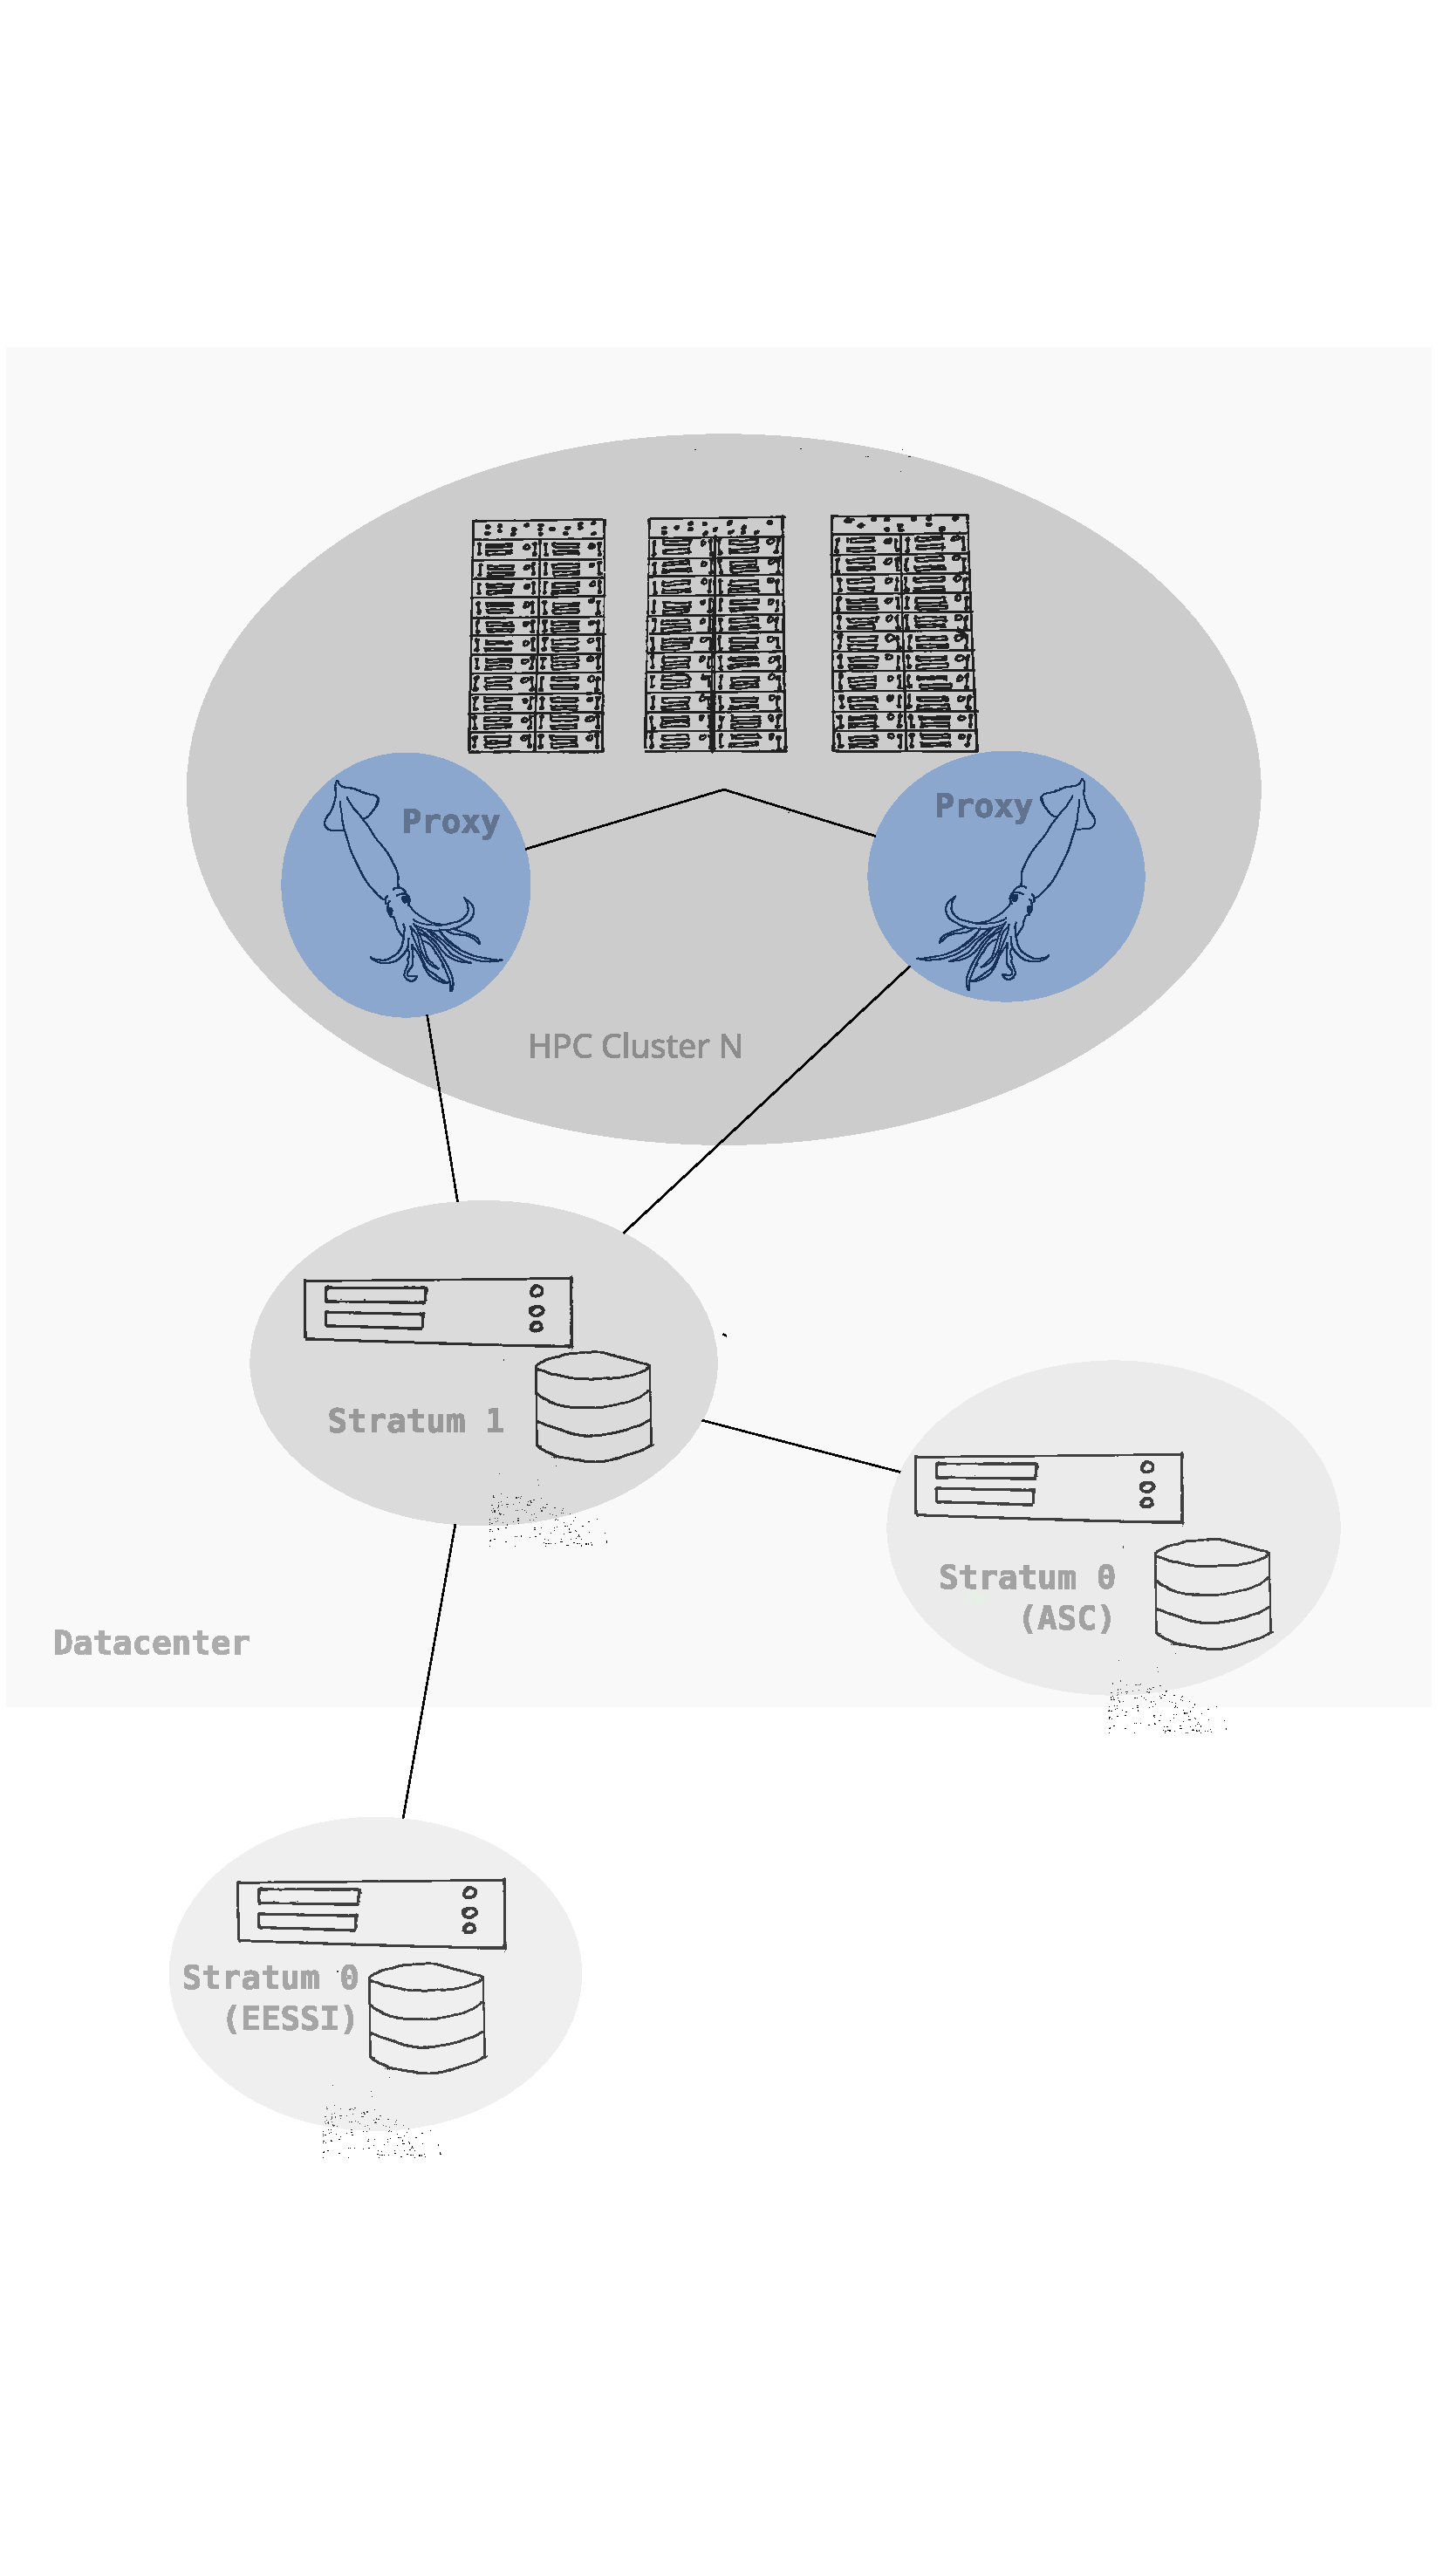
\includegraphics[width=280mm]{./include/main_cvmfs.pdf}
      \end{center}
    \end{block}
  \end{column}

  \begin{column}{0.48\textwidth}
      \begin{block}{Software built using EESSI-extend links against the compatibility layer}
        \lstinputlisting[language=bash]{./include/snippet-1.bash}
      \end{block}

      \begin{block}{Run time dependencies are resolved through software stack and compatibility layer}
        \lstinputlisting[language=bash]{./include/snippet-2.bash}
      \end{block}



      \begin{block} {Key challenges and observations}
          \begin{itemize}
            \item Implicit EasyBuild configuration is always loaded with EESSI-extend.
            \item EasyBlocks bundled with EESSI may not build cleanly under EESSI-extend.
            \item Cross-location side effects (e.g. user installs affecting site-wide setups) were observed.
            \item There will always be some interface to host (e.g. ofed
                libraries) this requires taking care to compile SLURM with
                  dependencies that are compatible with the MPI software
                  delivered with EESSI.
          \end{itemize}
      \end{block}

  \end{column}
\end{columns}

\vfill
\begin{block}{\centering \normalsize Tools and Technologies}
  \centering
  
\includegraphics[width=0.66\paperwidth]{./include/logos.pdf}
\end{block}

\end{frame}
\end{document}

